\section*{Exercise 2.1}
\enum{
\item
Since $\text{ran} X\subset\mathbb{N}$, then
\spl{
E[X]=\sum_{x=0}^{\infty}xP[X=x]=\sum_{x=0}^{\infty}\sum_{y=1}^{x}P[X=x].
}
We change the order of summation,
\spl{
    E[X]=\sum_{x=0}^{\infty}\sum_{y=1}^{x}P[X=x]=\sum_{x=0}^{\infty}\sum_{y=x+1}^{\infty}P[X=y]=\sum_{x=0}^{\infty}P[X>x].
}

\item 
According to the result we obtain in 1), we perform the similar calculation to $(X,f_X)$ where $X=1,2,\hdots,N-r+1$.
\spl{
    E[X]=\sum_{x=0}^{N-r}P[X>x].
}
In fact, $P[X>x]$ is equal to the probability that the first $x$ balls are all black.

\spl{
    P[X>x]&=P[\text{The first x balls are all black}]\\
    &=\frac{N-r}{N}\frac{N-r-1}{N-1}\hdots\frac{N-r-x+1}{N-x+1}\\
    &=\frac{(N-r)!/(N-r-x)!}{N!/(N-x)!}=\frac{\binom{N-x}{r}}{\binom{N}{r}}\\
    E[X]&=\frac{1}{\binom{N}{r}}\sum_{x=0}^{r'}\binom{N-x}{N-r'}=\frac{1}{\binom{N}{r}}\sum_{x=0}^{r'}\binom{N-r'+x}{N-r'}\\
    &=\frac{\binom{N+1}{N-r'+1}}{\binom{N}{r}}=\frac{\binom{N+1}{r+1}}{\binom{N}{r}}=\frac{N+1}{r+1}.
}
}

\section*{Exercise 2.2}
For $p_0(t)$, when $t=0$ the probability of 0 failure is 1. For $p_x(t)\quad (x\geq1)$, when $t=0$ the probability of x failure is 0.
Hence, the initial conditions are as the follows.
\spl{
    p_0(0)&=1\\
    p_{x}(0)&=0,\quad x\geq1.
}

Since $p_0'=-\lambda p_0$, then $p_0(t)=c\cdot e^{-\lambda t}$.
Also we know that $p_0(0)=1$, thus c=1.
Hence, $p_0(t)=e^{-\lambda t}$.

Assume that $p_x(t)=(\lambda t)^xe^{-\lambda t}/x!$ for all $x\in\mathbb{N}$.

For $x=0$, $p_0(t)=e^{-lambda t}=(\lambda t)^0e^{-\lambda t}/0!$, which follows our assumption.

For $x=n\geq0$, we assume the statement is true. When $x=n+1$,

\spl{
    &p_{n+1}'+\lambda p_{n+1}=\lambda p_n,\\
    &(e^{\lambda t}p_x)'=\lambda e^{\lambda t}p_n,\\
    &p_{n+1}=\frac{\int\lambda e^{\lambda t}p_n dt}{e^{\lambda t}}.
}
\spl{
    p_{n+1}&=\frac{\lambda e^{\lambda t}p_n dt}{e^{\lambda t}}=\frac{\int\lambda e^{\lambda t}(\lambda t)^ne^{-\lambda t}/n! dt}{e^{\lambda t}}\\
    &=\frac{\lambda^{n+1}/n! \int t^n dt}{e^{\lambda t}}=\lambda^{n+1}/n!/(n+1)(t^{n+1}+C)e^{-\lambda t}\\
    &=(\frac{(\lambda t)^{n+1}+(\lambda)^{n+1}C}{(n+1)!})e^{-\lambda t}.
}

To satisfy that $p_{n+1}(0)=0$, $C$ has to be 0. Thus,
\spl{
    p_{n+1}(t)=\frac{(\lambda t)^{n+1}}{(n+1)!}e^{-\lambda t}.
}

Therefore, $p_x(t)=(\lambda t)^xe^{-\lambda t}/x!$ for all $x\in\mathbb{N}$.

\section*{Exercise 2.3}
\spl{
    f(x)=\binom{n}{x}p^x(1-p)^{n-x}=\binom{n}{x}(\frac{k}{n})^x(1-\frac{k}{n})^{n-x}=k^x\frac{\binom{n}{x}}{n^x}((1-\frac{1}{n/k})^{n/k})^k(1-\frac{k}{n})^{-x}
}

Since
\spl{
    &\lim_{n\to\infty}\frac{\binom{n}{x}}{n^x}=\lim_{n\to\infty}\frac{n!}{x!(n-x)!n^x}=\frac{1}{x!},\\
    &\lim_{n\to\infty}((1-\frac{1}{n/k})^{-n/k})^{-k}=e^{-k},\\
    &\lim_{n\to\infty}(1-\frac{k}{n})^{-x}=1.
}

then
\spl{
    \lim_{n\to\infty}f(x)=\frac{k^x}{x!}e^{-k}.
}

\section*{Exercise 2.4}
\enum{
\item
\spl{
    E[V]&=\int_{0}^{\infty}(\frac{2}{\pi})^{1/2}(m/kT)^{3/2}v^3e^{-\frac{m}{kT}v^2/2}dv\\
    &=(\frac{2}{\pi})^{1/2}(m/kT)^{3/2}\int_{0}^{\infty}v^3e^{-\frac{m}{kT}v^2/2}dv\quad(w=v^2)\\
    &=(\frac{2}{\pi})^{1/2}(m/kT)^{3/2}\int_{0}^{\infty}w^{3/2}e^{-\frac{m}{kT}w/2}\frac{1}{2}w^{-1/2}dw\\
    &=(\frac{1}{2\pi})^{1/2}(m/kT)^{3/2}\int_{0}^{\infty}we^{-\frac{m}{kT}w/2}dw\\
    &=(\frac{m}{2kT\pi})^{1/2}\int_{0}^{\infty}\frac{m}{kT}we^{-\frac{m}{kT}w/2}dw\quad(z=-\frac{m}{kT}w/2)\\
}

\spl{
    E[V]=(\frac{8kT}{m\pi})^{1/2}\int_{-\infty}^{0}ze^zdz=(\frac{8kT}{m\pi})^{1/2}.
}

Since $Var[V]=E[V^2]-E[V]^2$, then
\spl{
    E[V^2]&=(\frac{2}{\pi})^{1/2}(m/kT)^{3/2}\int_{0}^{\infty}v^4e^{-\frac{m}{kT}v^2/2}dv\\
    &=-(\frac{2m}{k\pi T})^{1/2}\int_{1}^{0}v^3de^{-\frac{m}{kT}v^2/2}\\
    &=-(\frac{2m}{k\pi T})^{1/2}(v^3e^{-\frac{m}{kT}v^2/2}\bigg|_0^\infty-\int_0^\infty 3v^2e^{-\frac{m}{kT}v^2/2}dv)\\
    &=3(\frac{2m}{k\pi T})^{1/2}\int_0^\infty v^2e^{-\frac{m}{kT}v^2/2}dv\\
    &=3(\frac{2kT}{m\pi})^{1/2}\int_0^\infty e^{-\frac{m}{kT}v^2/2}dv\\
    &=\frac{3kT}{m}.
}

\spl{
    Var[V]=E[V^2]-E[V]^2=\frac{3kT}{m}-\frac{8kT}{m\pi}=\frac{kT}{m}(3-\frac{8}{\pi}).
}

\item
\spl{
    E[E]=E[mV^2/2]=mE[V^2]/2=\frac{3kT}{2}.
}

\item
Since
\spl{
    E&=\varphi(v)=\frac{mv^2}{2},\\
    V&=\varphi^{-1}(\varepsilon)=(\frac{2\varepsilon}{m})^{1/2},
}
then
\spl{
    f_E(\varepsilon)&=f_V(\varphi^{-1}(\varepsilon))\bigg|\frac{d\varphi^{-1}(\varepsilon)}{d\varepsilon}\bigg|=(\frac{1}{2m\varepsilon})^{1/2}(\frac{2}{\pi})^{1/2}(\frac{m}{kT})^{3/2}\frac{2\varepsilon}{m}e^{-\frac{\varepsilon}{kT}}\\
    &=2(\frac{\varepsilon}{\pi k^3T^3})^{1/2}e^{-\frac{\varepsilon}{kT}}. 
}

}

\section*{Exercise 2.5}
\spl{
    \Gamma(\frac{2n+1}{2})&=\int_0^\infty t^{(2n-1)/2}e^{-t}dt=(t^{(2n-1)/2}e^{-t})\bigg|_0^\infty+\frac{2n-1}{2}\int_0^\infty t^{(2n-3)/2}e^{-t}dt\\
    &=(\frac{2n-1}{2})\Gamma(\frac{2n-1}{2}).
}

Hence,
\spl{
    \Gamma(\frac{2n+1}{2})=\frac{(2n-1)(2n-3)\hdots(1)}{2\cdot2\hdots2}\Gamma(\frac{1}{2})=\frac{(2n-1)!!}{2^n}\Gamma(\frac{1}{2}).
}

Also we obtain
\spl{
    \Gamma(\frac{1}{2})&=\int_0^\infty t^{-1/2}e^{-t}dt\quad(t=w^2)\\
    &=\int_0^\infty w^{-1}e^{-w^2}2wdw=2\int_0^\infty e^{-w^2}dw=\sqrt{\pi}
}

Therefore,
\spl{
    \Gamma(\frac{2n+1}{2})=\frac{(2n-1)!!}{2^n}\sqrt{\pi}.
}

\section*{Exercise 2.6}
\enum{
\item
Denote that
\spl{
    Z=\frac{X-\mu}{\sigma}=\frac{X-6000}{100}
}
so that $Z\sim N(0,1)$.
Then,
\spl{
    &P[\text{A sample strength is less than 6250 kg/cm$^2$}]\\
    &=P[X<6250]=P[Z<2.50]=\Phi(2.50)=0.9938.
}

\item
\spl{
    P[5800\leq X\leq 5900]&=P[-2.00\leq Z\leq -1.00]\\
    &=\Phi(-1.00)-\Phi(-2.00)\\
    &=0.1587-0.0228\\
    &=0.1359.
}

\item
According to the standard normal distribution table, we know that
\spl{
    \Phi(-1.64)=0.0505,\quad \Phi(-1.65)=0.0495.
}

When $Z=-1.65$, $X=-1.65\times100+6000=5835$kg/cm$^2$.

Hence, the strength of 5835 kg/cm$^2$ exceeds 5\% samples, saying that is exceeded by 95\% samples.
}

\section*{Exercise 2.7}
\enum{
\item
The random variable is a map $X:\ S\to \mathbb{R}$ together with a function $f_X:\ \mathbb{R}\to\mathbb{R}$. Then, the two properties of a continuous random variable will be showed.

For $a<x<b$ where $b>a$, $f(x)=1/(b-a)>0$.
For other conditions, $f(x)=0>=0$.
Hence, $f(x)\geq0$.

Also,
\spl{
    \int_{-\infty}^{\infty}f(x)dx=\int_{a}^{b}1/(b-a)dx=(b-a)/(b-a)=1.
}

Hence, this is a density for a continuous random variable.

\item
The graph is as the following.
\begin{figure}[H]
    \centering
    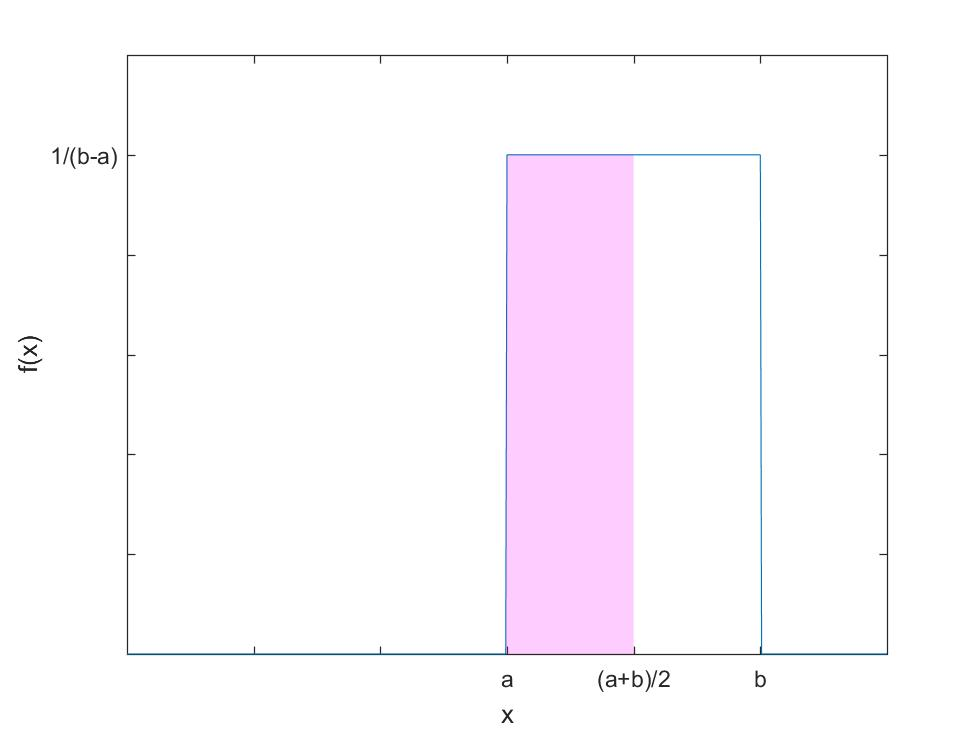
\includegraphics[height=5.5cm]{images/a}
    \caption{Graph for Exercise 2.7 (2)}
\end{figure}

\item
\spl{
    P[X<=(a+b)/2]=\int_{-\infty}^{(a+b)/2}f(x)dx=\int_{a}^{(a+b)/2}1/(b-a)dx=(b-a)/2/(b-a)=\frac{1}{2}.
}

\item
Since [c,d] and [e,f] are the subintervals of [a,b], then
\spl{
    P[c\leq X\leq d]&=\int_{c}^{d}1/(b-a)dx=(d-c)/(b-a).\\
    P[e\leq X\leq f]&=\int_{e}^{f}1/(b-a)dx=(f-e)/(b-a).
}

Since $d-c=f-e$, then $P[c\leq X\leq d]=P[e\leq X\leq f]$.

\item
\[
    F(x)=\int_{-\infty}^{x}f(t)dt=
    \left\{\begin{aligned}
        &0,\quad x<a\\
        &\frac{x-a}{b-a},\quad a\leq x \leq b\\
        &1,\quad x>b\\
    \end{aligned}\right.
\]

\item
\spl{
    E[X]&=\int_{-\infty}^{\infty}xf(x)dx=\int_{a}^{b}\frac{x}{b-a}dx\\
    &=\frac{x^2}{2(b-a)}\bigg|_a^b=\frac{b^2-a^2}{2(b-a)}=\frac{a+b}{2}.
}
\spl{
    E[X^2]&=\int_{-\infty}^{\infty}x^2f(x)dx=\int_{a}^{b}\frac{x^2}{b-a}dx\\
    &=\frac{x^3}{3(b-a)}\bigg|_a^b=\frac{b^3-a^3}{3(b-a)}=\frac{a^2+ab+b^2}{3}. 
}
Hence,
\spl{
    Var[X]&=E[X^2]-E[X]^2=\frac{a^2+ab+b^2}{3}-(\frac{a+b}{2})^2\\
    &=\frac{(b-a)^2}{12}.
}
}